\begin{figure}[H]
	\centering
	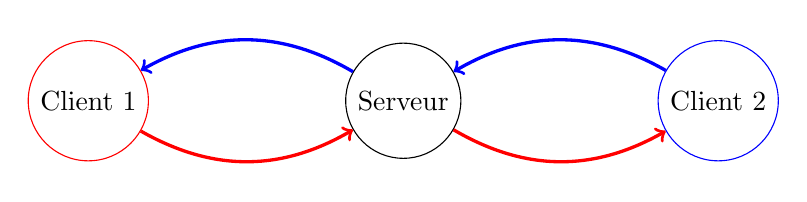
\begin{tikzpicture}
		\begin{scope}[every node/.style={circle, draw}]
			\node (S) at (0,0) {Serveur};
			\node[draw=red] (C1) at (-4,0) {Client 1};
			\node[draw=blue] (C2) at (4,0) {Client 2};
		\end{scope}
		\begin{scope}[every edge/.style={draw=red, very thick, bend right=30}]
			\path [->] (C1) edge node {} (S);
			\path [->] (S) edge node {} (C2);
		\end{scope}
		\begin{scope}[every edge/.style={draw=blue, very thick, bend right=30}]
			\path [->] (C2) edge node {} (S);
			\path [->] (S) edge node {} (C1);
		\end{scope}
	\end{tikzpicture}
	\caption{Une représentation abstraite du modèle client-serveur}
	\label{fig:repr-serveur}
\end{figure}

Comme le montre le graphe dans la figure~\ref{fig:repr-serveur}, 
chaque client $x$ communique au serveur, puis ce que le client $x$ communique au serveur est retranscrit  aux autres clients.
Cela implique deux choses. Premièrement, un isolement des responsabilités. En effet, le serveur
et les clients ne font pas du tout la même chose. Le serveur fait le principal du travail tandis que les clients jouent.
Deuxièmement, il faut une langue commune. En effet, si le client 1 parle anglais, tandis que le serveur parle espagnol et le client 2 russe,
ils ne se comprendront pas\footnote{Sauf coup de chance extrême}. Cette idée de langue
commune s'appelle une \emph{interface} en programmation. Il faut une interface
commune à chaque client entre clients et serveurs. Cette interface nous a été fourni par le sujet. Cela permet
de faire jouer les clients des différentes équipes dans un tournoi.

\subsection{Isolation des responsabilités}

Le serveur s'occupe de lancer la partie, de la dérouler, et de déterminer la terminaison de la partie.
Pour avoir un bon déroulement de la partie et permettre aux clients de jouer,
il doit informer le prochain client à jouer du coup joué par le client précédent.
Les clients, eux, doivent \emph{correctement} jouer à la partie.

On remarque que le serveur et les clients ont besoin de garder en mémoire l'évolution d'une partie.
Le serveur en a besoin pour savoir si un joueur fait un coup invalide.
Les clients en ont besoin pour suivre une stratégie cohérente.

On décide donc de créer un troisième module nommé \verb|common| qui implémentera toutes les fonctionnalités communes 
aux clients et au serveur.

\subsection{Interface entre client et serveur}

Les clients doivent disposer de quatres fonctions.
\begin{itemize}
    \item \textbf{get\_player\_name()} : Retourne le nom du joueur.
    \item \textbf{initialize(plateau)} : Permet au joueur de se préparer pour la partie à venir.
    \item \textbf{play(coup\_precedent)} : Indique au joueur quel coup l'autre client a joué et demande au joueur de jouer un coup.
    \item \textbf{finalize()} : Permet au joueur de libérer les ressources allouées.
\end{itemize}

Cette interface établie une généricité entre tous les clients et permet de les faire s'affronter.
Cela rend possible la création d'une compétition pour établir quelle est 
la meilleur stratégie.